\documentclass{article}
\usepackage[utf8]{inputenc}
\usepackage{graphicx}
\usepackage{mathtools}
\usepackage{amssymb}
\usepackage{amsmath}
\usepackage{macros}
\usepackage{color}

\begin{document}

\section{TATA41 - Föreläsning 3}

\section{Standardgränsvärden}

\subsection{Exempel}
$$ f(x) = \f{\sin(x)} x, x\neq 0 $$
$$ f(-x) = \f{\sin(-x)}{-x} = f(x), x\neq 0 $$
($f$ är en jämn funktion (spegelsymmetri).)

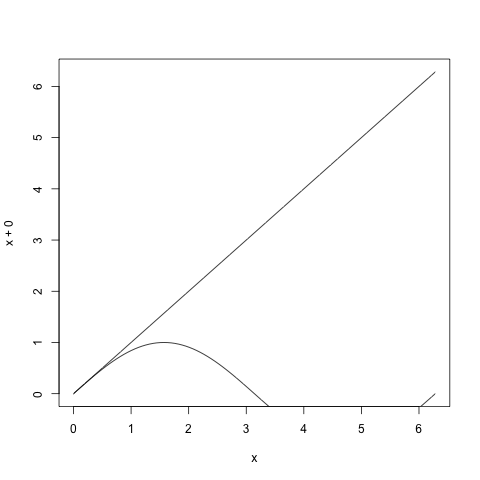
\includegraphics[height=60mm, width=60mm]{img/xsinx.png}
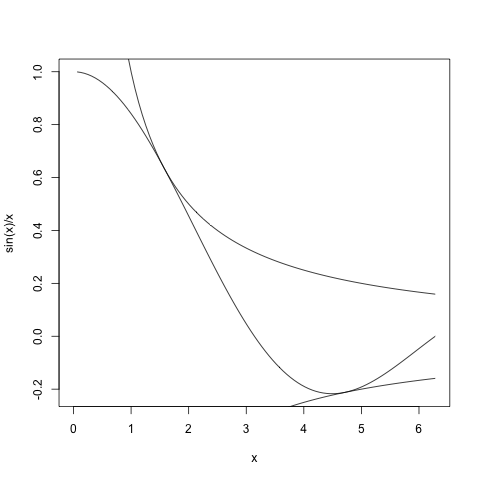
\includegraphics[height=60mm, width=60mm]{img/sinxx.png}
\subsection{Sats}
Om $c>0$ och $a>1$ så gäller följande:\\
\subsubsection{a}
$$\lm x 0 \f{\sin(x)}{x} = 1$$
\subsubsection{b}
$$\lm x 0 \f{\ln(1+x)}{x} = 1$$
\subsubsection{c}
$$\lm x 0 \f{e^x - 1}{x} = 1$$
\subsubsection{d}
$$\lm{x}{0^+} x^c \times \ln(x) = 0$$
\subsubsection{e}
$$\lm{x}{\infty} \f{x^c}{\ln x} = \infty$$
och därmed
$$\lm{x}{\infty} \f{\ln x}{x^c} = 0$$
\subsubsection{f}
$$\lm{x}{\infty} \f{a^x}{x^c} = \infty$$

\subsection{Bevis}
\subsubsection{a}
Antag först att $0<x<\f \pi x$. Från grunken vet vi då att
$$ 0 < \sin x < x < \tan x $$
Division med $\sin x$ (positivt) ger $=\f{\sin x}{\cos x}$
$$ 0 < 1 < \f x{\sin{x}} < \f 1{\cos{x}} $$
alltså (eftersom $0<a<b\eq 0<\f 1b <\f 1a$):
$$ \cos x < \f{\sin x}x<1 $$
Vi vet att:
$$ \cos x \to 1, x \to 0 $$
Enligt instängningsregeln ger
$$ \f{\sin x}x \to 1, x\to 0^+$$

\subsubsection{b}
Från grunken:
$$ \f{t-1}t \le \ln t \le t-1, t>0 $$

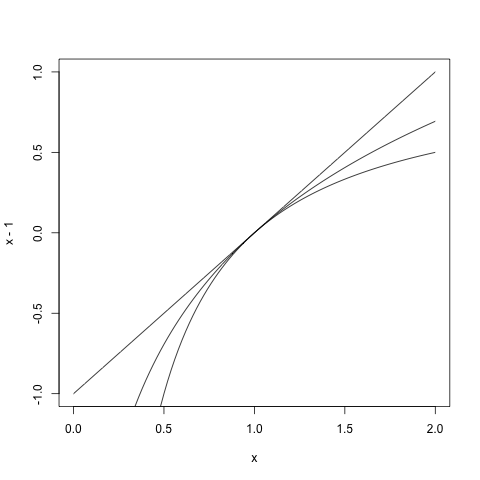
\includegraphics[height=60mm, width=60mm]{img/lntt.png}

Alltså, med $t=1+x$
$$ \f x{x+1} \le \ln(1+x) \le x, x>-1 $$

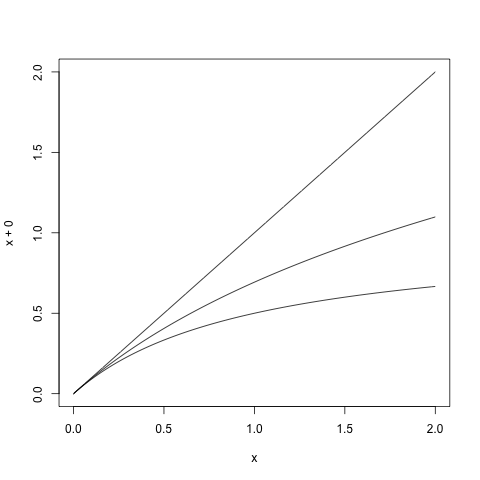
\includegraphics[height=60mm, width=60mm]{img/lntt1.png}

För $x>0$
$$ \f 1{1+x} \le \f{\ln(1+x)}x \le 1 \im \f{\ln(1+x)}x \to 1, x\to 0^+ $$\\
För $x<0$
$$ \f 1{1+x} \ge \f{\ln(1+x)}x \ge 1 \im \f{\ln(1+x)}x \to 1, x\to 0^- $$

\subsubsection{c-f}
Se boken.

\subsection{Exempel}
$$ \f{\sin 4x}{\sin 3x} = \f{\sin 4x}{4x} \times \f{3x}{\sin 3x} \times \f 43 \to 1\times 1\times \f 43 = \f 43, x\to 0 $$
(enligt standardgränsvärden)

\subsection{Exempel}
$$ \f{\ln x + 7}{e^x - 5} = \f{\ln x \times (1 + \f 7{\ln x})}{e^x\times (1-\f 5{e^x})} =
\f{\ln x} x \times \f{x}{e^x} \times \f{(1 + \f 7{\ln x})}{(1-\f 5{e^x})} \to 0, x\to\infty$$

\subsection{Exempel}
Undersök
$$ \lm x 1 \f { e^{\cos(\f{x\pi}2) - x} }{ \ln x } $$
Lösning: Sätt $x = 1+t$ (obs att $x\to 1 \eq t\to 0$).\\
Då blir $\cos(\f{x\pi}2) = \cos(\f{\pi (1+t)}2) = \cos(\f \pi 2 + \f{t\pi}2) = -\sin(\f{t\pi}2)$\\
Så
$$
\f{e^{\cos(\f{x\pi}2)} - x}{\ln x} = \f{e^{-\sin(\f{t\pi}2)} - (1+t)}{\ln (1+t)} =
$$
$$
\f{e^{-\sin(\f{t\pi}2)} - 1}{\ln (1+t)} - \f t{\ln(1+t)}=
$$
$$
\f{e^{-\sin(\f{t\pi}2)} - 1}{-\sin{\f{t\pi}{2}}} \times \f{-\sin{t\pi}2}{\f{t\pi}2} \times \f{\f{t\pi}2}{\ln(1+t)} - \f t{\ln(1+t)} \to
$$
$$
1 \times (-1)\times \f \pi 2 \times 1 = -\f \pi 2 - 1, t\to 0, (x\to 1)
$$

\section{Talföljder}
\subsection{Notation}
$$ (a_n)^\infty_{n=0} = (a_0, a_1, a_2, \cdots) $$

\subsection{Definition}
Om $\lm n \infty a_n$ existerar (ändligt) så kallas följden konvergent, annars divergent.

\subsection{Sats}
\subsubsection{a}
$$\lm n \infty \f{a^n}{n!} = 0$$
\subsubsection{b}
$$\lm n \infty \f{n!}{n^n} = 0$$

\subsubsection{c}
$$\lm n \infty n^{1/n} = 1$$

\subsection{Bevis}
\subsubsection{a och b}
Se boken.

$$ a^{n} = a\times a\times a \times \cdots \times a $$
$$ n! = 1\times 2\times 3\times \cdots\times n$$
$$ n^n = n\times n\times n\times \cdots \times n $$

\subsubsection{c}
$$ n^{1/n} = (e^{\ln n \times n})^{1/n} = e^{\ln n \times \f 1n}= e^{\f{\ln n}{n} \to e^0 = 1, n\to \infty} $$

\subsection{Kluring/övning}
Visa
$$ \lm n \infty (n!)^{1/n} = \infty $$

\subsection{Anmärkning}
Stirlings approximation säger
$$ n! \approx \sqrt{2\pi n} \times (\f ne)^n \times e^{\f 1{12n}} $$

\subsection{Sats}
Antag att följden $ (a_n)^\infty_{n=1}$ är växande och uppåt begränsad, dvs
$$ a_1 \le a_2 \le a_3 \le \cdots \le C $$
För någon konstatn C.\\
Då existerar $A = \lm n \infty a_n$ (ändligt)

\subsection{Bevis}
Appendix A

\end{document}
